\chapter{Hydrodynamic Design Optimisation}
\label{ch: captive design optimisation}



% \begin{figure}[h]
%     \centering
%     \begin{subfigure}[b]{0.49\textwidth}
%         \centering
%         \includegraphics[width=\textwidth]{}
%         \caption[]%
%         {{\small }}    
%         \label{fig:  }
%     \end{subfigure}
%     \hfill
%     \begin{subfigure}[b]{0.49\textwidth}  
%         \centering 
%         \includegraphics[width=\textwidth]{}
%         \caption[]%
%         {{\small }}    
%         \label{fig:  }
%     \end{subfigure}
%     \vskip\baselineskip
%     \begin{subfigure}[b]{0.49\textwidth}   
%         \centering 
%         \includegraphics[width=\textwidth]{}
%         \caption[]%
%         {{\small }}    
%         \label{fig:  }
%     \end{subfigure}
%     \hfill
%     \begin{subfigure}[b]{0.49\textwidth}   
%         \centering 
%         \includegraphics[width=\textwidth]{}
%         \caption[]%
%         {{\small }}    
%         \label{fig:  }
%     \end{subfigure}
%     \hfill
%     \begin{subfigure}[b]{0.49\textwidth}   
%         \centering 
%         \includegraphics[width=\textwidth]{}
%         \caption[]%
%         {{\small }}    
%         \label{fig:  }
%     \end{subfigure}
%         \hfill
%     \begin{subfigure}[b]{0.49\textwidth}   
%         \centering 
%         \includegraphics[width=\textwidth]{}
%         \caption[]%
%         {{\small }}    
%         \label{fig:  }
%     \end{subfigure}
    
%     \caption{}
%     \label{fig: }
% \end{figure}

In this chapter, an optimisation of the design of a breakwater geometry for a captive set-up is presented. A 'captive' setup means that all motions of the structure are restrained. The performance of each breakwater is determined in ComFLOW for 300 seconds simulation time. The first design iteration of the optimisation is performed for Wave Condition 1 (regular waves of H = 3.0 m and T = 6.0 s) and is discussed in Section \ref{sec: design iteration 1 captive}. The results are used to do a second design iteration with boundaries around the optimum of the first design iteration; this is addressed in Section \ref{sec: design iteration 2 captive}. The effect of Wave Condition 2 on the optimal designs is shown in Section \ref{sec: WC2 captive}. Here, the performance of the breakwaters is tested for extreme, regular waves with a height of 9 metres and a peak period of 10.4 seconds. Finally, a more extensive analysis of the results is performed in the final section: \ref{sec: discussion hydrodynamical optimisation}, where an explanation of the results is further analysed based on physical phenomena and the literature. 


% An optimisation based on costs is done in the sections \ref{sec: economical DI1 H3} and \ref{sec: economical DI2 H3} for Wave Condition 1. Finally, the results of the captive design optimisation are discussed in Section \ref{sec: discussion captive design optimization} and conclusions are drawn in Section \ref{sec: conclusions captive design optimization}.
%and sometimes two design iterations are necessary to deliver the optimal design




\section{Design Iteration 1}
\label{sec: design iteration 1 captive}

The first design iteration of the captive set-up is addressed in this section. In Section \ref{sec: DI1 captive H3 approach} the approach is declared, the performance of all the breakwaters in the design space is discussed in Section \ref{sec: DI1 captive H3 performance bw}, in Section \ref{sec: DI1 captive H3 correlation} the correlation between input factors and responses are discussed in Section \ref{sec: DI1 captive H3 response surfaces} the response surfaces are shown, which are used to arrive at the final design optima, which are reported in the final section; \ref{sec: DI1 captive H3 design optima}.


\subsection{Approach}
\label{sec: DI1 captive H3 approach}

In the first design iteration, various configurations of breakwaters are simulated in ComFLOW with varying factors. The limits of these factors are shown in Table \ref{tab: boundaries DI1 captive}. A clarification on how these factors define the actual geometry of the breakwater is explained in Section \ref{subsec: methodology parametrisation} of the \nameref{ch: methodolgy} chapter and visualised in Figure \ref{fig: parametrisation breakwater}. Also, a minimal clearing of 10 metres between the seabed and the bottom of the breakwater is implemented in Design Expert (i.e. the maximum draught is 13 metres, because the water depth is 23 metres), otherwise large fluid velocities below the breakwater were expected, that result in low pressure fields and long execution times. A cubic relation between all the different input parametres and the two responses: the mean drift force and the transmitted wave height, is assumed. To be able to construct the response surfaces, 94 configurations are necessary to be simulated in ComFLOW. With the help of \acrfull{doe} a design space is created, which defines the shape of the 94 configurations. The complete design space is given in Appendix Table \ref{tab: params design iteration 1 captive setup}. To show the variety of the possible geometries of the breakwaters, the parametres for six different configurations are shown in Table \ref{tab: params design iteration 1 captive br 1to6} and are visualised in Figure  \ref{fig:Configurations 1to6 DI1 captive}. Evidently, the breakwaters vary from small wedges completely submerged to big boxes on the surface. 

\begin{table}[h]
\centering
\scalebox{0.65}{
\begin{tabular}{@{}ccccc@{}}
\toprule
Factor & Name        & Units        & Minimum & Maximum       \\ \midrule
A & T               & m & 2.50   & 13.00   \\
B & W               & m & 10.00  & 150.00   \\
C & front\_fraction & - & 0.01 & 0.99  \\
D & top\_fraction   & - & 0.01 & 0.99  \\
E & radius          & m & 500.00 & 2000.00 \\
F & WL              & m & -6.10  & 4.00     \\ \bottomrule
\end{tabular}
}
\caption{Boundaries Design Space Captive Design Iteration 1}
\label{tab: boundaries DI1 captive}
\end{table}

% Please add the following required packages to your document preamble:
% \usepackage{booktabs}
\begin{table}[h]
\centering
\scalebox{0.65}{
\begin{tabular}{@{}ccccccc@{}}
\toprule
configuration & T        & W        & front\_fraction & top\_fraction & radius   & WL       \\ \midrule
16 & 9.59 & 150.00      & 0.01   & 0.01   & 2000.00   & 3.41 \\
24 & 5.44     & 89.80     & 0.01   & 0.2795 & 1985.00   & -3.37   \\
32 & 8.64   & 10.00       & 0.01   & 0.01   & 500.00    & 4.00        \\
37 & 12.30 & 150.00      & 0.85 & 0.5539 & 920.00    & -0.70 \\
40 & 7.75     & 41.16 & 0.99   & 0.79 & 852.50  & -2.87   \\
45 & 2.50      & 150.00      & 0.64 & 0.99   & 1272.5 & 2.18    \\ \bottomrule
\end{tabular}
}
\caption{Parametres breakwater of six different configurations of design iteration 1}
\label{tab: params design iteration 1 captive br 1to6}
\end{table}

\begin{figure}[h]
    \centering
    \begin{subfigure}[b]{0.49\textwidth}
        \centering
        \includegraphics[width=\textwidth]{figures/ComFLOW/Breakwater Geometries/Design Iteration 1 captive/general/breakwater_geometry24.pdf}
        \caption[]%
        {{\small}configuration 24}    
        \label{fig: It1 Configuration 16}
    \end{subfigure}
    \hfill
    \begin{subfigure}[b]{0.49\textwidth}  
        \centering 
        \includegraphics[width=\textwidth]{figures/ComFLOW/Breakwater Geometries/Design Iteration 1 captive/general/breakwater_geometry45.pdf}
        \caption[]%
        {{\small}configuration 45}    
        \label{fig: It1 Configuration 24}
    \end{subfigure}
    \vskip\baselineskip
    \begin{subfigure}[b]{0.49\textwidth}   
        \centering 
        \includegraphics[width=\textwidth]{figures/ComFLOW/Breakwater Geometries/Design Iteration 1 captive/general/breakwater_geometry16.pdf}
        \caption[]%
        {{\small}configuration 16}    
        \label{fig: It1 Configuration 32}
    \end{subfigure}
    \hfill
    \begin{subfigure}[b]{0.49\textwidth}   
        \centering 
        \includegraphics[width=\textwidth]{figures/ComFLOW/Breakwater Geometries/Design Iteration 1 captive/general/breakwater_geometry37.pdf}
        \caption[]%
        {{\small}configuration 37}    
        \label{fig: It1 Configuration 37}
    \end{subfigure}
    \hfill
    \begin{subfigure}[b]{0.49\textwidth}   
        \centering 
        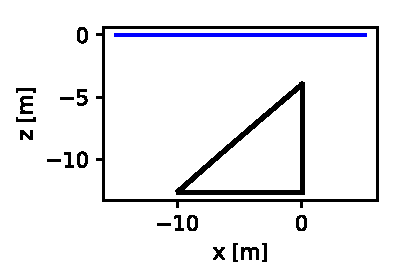
\includegraphics[width=0.5\textwidth]{figures/ComFLOW/Breakwater Geometries/Design Iteration 1 captive/general/breakwater_geometry32.pdf}
        \caption[]%
        {{\small}configuration 32}    
        \label{fig: It1 Configuration 40}
    \end{subfigure}
        \hfill
    \begin{subfigure}[b]{0.49\textwidth}   
        \centering 
        \includegraphics[width=\textwidth]{figures/ComFLOW/Breakwater Geometries/Design Iteration 1 captive/general/breakwater_geometry40.pdf}
        \caption[]%
        {{\small}configuration 40}    
        \label{fig: It1 Configuration 45}
    \end{subfigure}
    
    \caption{Six different configurations of the first design iteration}
    \label{fig:Configurations 1to6 DI1 captive}
\end{figure}


The performance of each breakwater is quantified after all configurations of the design space were simulated in ComFLOW by studying the influence of the magnitude of the factors (T, W, front\_fraction, top\_fraction and WL) on the responses (mean wave drift force and wave transmission). The mean wave drift force is nondimensionalised by dividing it through the mean wave load on a wall, this quantity is called $F_{d,norm}$ (equation \ref{eq: handling Fdnorm}). Wave transmission is studied through the wave transmission coefficient $K_t$, which is the ratio between the transmitted wave height and the incident wave height. Note again that the factor WL, which defines the position z of the breakwater, shifts the waterline with regard to the origin of the body-fixed coordinate system (see Figure \ref{fig: parametrisation breakwater}), which is on top of the breakwater behind the sloping beach (see Figure \ref{fig: parametrisation breakwater}). For example, with WL = 1 the top of the breakwater is one metre below the waterline and WL = -1 means one metre of the breakwater is above the waterline.




\subsection{Performance breakwaters}
\label{sec: DI1 captive H3 performance bw}

% -performance breakwaters mapped to plot their mean wave drift force wrt wave transmission
% -configuration 5 probably a unreasonably low mean wave drift force. 
% -best performing at wave attenuation are large boxes underneath close to waterline, it is expected. Expected by literature (linear wave theory)
% -best at having a low mean wave drift force are large wedge-type structures. Expected by literature--> dissipation leads to lowering mean wave drift force

The performance of the 94 breakwaters of the design space of this first design iteration is mapped in Figure \ref{fig: Fd vs. Kt DI1 H3 captive}, where the normalised mean wave drift force (F$_{d,norm}$) is plotted against the wave transmission coefficient (K$_t$ = H$_t$/H$_i$). Figure \ref{fig: Fd vs. Kt DI1 H3 captive pareto} is zoomed in on the Pareto front (the set of most efficient solutions in a multi-objective optimisation) and the shape of these best performing breakwaters is shown in Figure \ref{fig: pareto front bw DI1 H3 captive}. The breakwaters that perform best in attenuating wave energy on this Pareto front are very large box-type structures (high depth and width) and are placed around the waterline with their top. Those on the Pareto front best at minimising the mean wave drift force are structures placed further beneath the water surface and possess a sloping beach which induces the incoming waves to break and thereby dissipate wave energy.  


Note that configuration 5 is not included in the Pareto front, because it gave results from which it is not sure whether this is an accurate representation of reality. The average water level of the simulation of this breakwater is shown in Figure \ref{fig: average wl configuration 5}, from which can be seen that a large set-down of the water level is present in front of the structure. This is caused by a downwards fluid flow, shown in Figure \ref{fig: fluid flow configuration 5}. Over time can be seen that the waves break on the breakwaters surface, after which the fluid particles on top flow back (into the direction of negative x) and once the fluid particles flow over the edge they are sucked to the bottom of the domain. This causes a low pressure region and this might be the reason the geometry has experiences a very low mean wave drift force over time. 

\begin{figure}[h]
    \centering
    \begin{subfigure}[b]{0.49\textwidth}
        \centering
        \includegraphics[width=\linewidth]{figures/ComFLOW/Results DI1/Fd_norm_VS_Kt_normal.pdf}
        \caption[]%
        {{\small All breakwaters}}    
        \label{fig: Fd vs. Kt DI1 H3 captive normal}
    \end{subfigure}
    \hfill
    \begin{subfigure}[b]{0.49\textwidth}  
        \centering 
        \includegraphics[width=\linewidth]{figures/ComFLOW/Results DI1/Fd_norm_VS_Kt_Pareto.pdf}
        \caption[]%
        {{\small Pareto front}}    
        \label{fig: Fd vs. Kt DI1 H3 captive pareto}
    \end{subfigure}
    
    \caption{Mean wave drift force Vs. Wave transmission}
    \label{fig: Fd vs. Kt DI1 H3 captive}
\end{figure}




\begin{figure}[h]
    \centering
    \begin{subfigure}[b]{0.49\textwidth}
        \centering
        \includegraphics[width=\linewidth]{figures/ComFLOW/Breakwater Geometries/Design Iteration 1 captive/general/breakwater_geometry5.pdf}
        \caption[]%
        {{\small Configuration 5}}    
        \label{}
    \end{subfigure}
    \hfill
    \begin{subfigure}[b]{0.49\textwidth}  
        \centering 
        \includegraphics[width=\linewidth]{figures/ComFLOW/Breakwater Geometries/Design Iteration 1 captive/general/breakwater_geometry37.pdf}
        \caption[]%
        {{\small Configuration 37}}    
        \label{}
    \end{subfigure}
    
    \centering
    \begin{subfigure}[b]{0.49\textwidth}
        \centering
        \includegraphics[width=\linewidth]{figures/ComFLOW/Breakwater Geometries/Design Iteration 1 captive/general/breakwater_geometry45.pdf}
        \caption[]%
        {{\small Configuration 45}}    
        \label{}
    \end{subfigure}
    \hfill
    \begin{subfigure}[b]{0.49\textwidth}  
        \centering 
        \includegraphics[width=\linewidth]{figures/ComFLOW/Breakwater Geometries/Design Iteration 1 captive/general/breakwater_geometry1.pdf}
        \caption[]%
        {{\small Configuration 1}}    
        \label{}
    \end{subfigure}
    
    \centering
    \begin{subfigure}[b]{0.49\textwidth}
        \centering
        \includegraphics[width=\linewidth]{figures/ComFLOW/Breakwater Geometries/Design Iteration 1 captive/general/breakwater_geometry71.pdf}
        \caption[]%
        {{\small Configuration 71}}    
        \label{}
    \end{subfigure}
    
    \caption{Wave breakers on Pareto front}
    \label{fig: pareto front bw DI1 H3 captive}
\end{figure}



\begin{figure}[h]
    \centering
    \begin{subfigure}[b]{0.49\textwidth}
        \centering
        \includegraphics[width=\linewidth]{figures/ComFLOW/Results average wl/configuration5.pdf}
        \caption[]%
        {{\small Average water level}}    
        \label{fig: average wl configuration 5}
    \end{subfigure}
    \hfill
    \begin{subfigure}[b]{0.49\textwidth}  
        \centering 
        \includegraphics[width=\linewidth]{figures/ComFLOW/Results DI1/config_5_run_23.png}
        \caption[]%
        {{\small Downwards fluid flow in front of breakwater}}    
        \label{fig: fluid flow configuration 5}
    \end{subfigure}
    
    \caption{Visualisation of low pressure field in front of configuration 5}
    \label{fig: configuration 5 low pressure field }
\end{figure}





\subsection{Correlation}
\label{sec: DI1 captive H3 correlation}


Figure \ref{fig: correlation DI1 captive} shows the correlation between all the factors and responses. Where red means a positive correlation and blue a negative. So, from this Figure can be concluded a large floater width $W$ leads to a small transmission coefficient $K_t$ and a deeply submerged breakwater (high $WL$) leads to a high wave transmission but low mean wave drift force. Figures \ref{fig: perturbation R1 DI1 captive} and \ref{fig: perturbation R2 DI1 captive} show the trend of the a change in factors (A to F) on respectively the mean wave drift force (Fd\_norm) and the transmitted wave height (Kt$^2$).\\
\\
Figures \ref{fig: perturbation R1 DI1 captive} shows that the mean wave drift force is negatively correlated with the z position of the breakwater (factor F), with its minimum around 1.5 metres below the waterline. This correlation is present for the largest part of the spectrum, but there is a positive correlation at the boundaries (i.e. its maximum and minimum lie within the design space boundaries). The same trend is observed in Figure \ref{fig: Fd_norm_VS_top_bw_with_Kt DI1 captive H3}, where the mean wave drift force of the breakwaters of the design space is plotted against the z position of the body-fixed origin w.r.t. the waterline. From this Figure can be seen that most submerged breakwaters experienced a negative mean wave drift force, while some of them also have good wave attenuation performance. \\
Also, the correlation between factor F and the wave transmission  coefficient (figure \ref{fig: perturbation R2 DI1 captive}) shows that breakwaters where the origin of the body-fixed coordinate system is placed between 0 and 2 metres above the water level perform best, at attenuating wave energy. When the breakwater would be placed higher or lower than this optimum, it would perform less (higher $K_t$), with a stronger correlation when factor F rises (i.e. while the breakwater will be positioned deeper, its wave attenuating performance decreases significantly). Also, in this Figure could be observed the negative correlation between the floater width (factor B) and the wave transmission is stronger for small floater widths.\\
Furthermore, the wave transmission $K_t$ has a negative correlation with the mean wave drift force $F_{d,norm}$. In other words, when a large mean wave drift force occurs a small transmission coefficient is present, on average. 



\begin{figure}[h]
    \centering
    \begin{subfigure}[b]{0.30\textwidth}  
        \centering 
        \includegraphics[width=\linewidth]{figures/ComFLOW/Results DI1/correlation.png}
        \caption[]%
        {{\small Correlation between factors and responses}}    
        \label{fig: correlation DI1 captive}
    \end{subfigure}
    \hfill
    \begin{subfigure}[b]{0.49\textwidth}
        \centering
        \includegraphics[width=\linewidth]{figures/ComFLOW/Results DI1/Fd_norm_VS_top_bw_with_Kt.pdf}
        \caption[]%
        {{\small Mean wave drift force to z-positioning breakwaters}}    
        \label{fig: Fd_norm_VS_top_bw_with_Kt DI1 captive H3}
    \end{subfigure}

    \caption{}
    \label{fig: }
\end{figure}    
    
\begin{figure}[h]
    \centering
    \begin{subfigure}[b]{0.49\textwidth}
        \centering
        \includegraphics[width=\linewidth]{figures/ComFLOW/Results DI1/perturbation R1.pdf}
        \caption[]%
        {{\small Perturbation Response 1: Mean wave drift force}}    
        \label{fig: perturbation R1 DI1 captive}
    \end{subfigure}
    \hfill
    \begin{subfigure}[b]{0.49\textwidth}  
        \centering 
        \includegraphics[width=\linewidth]{figures/ComFLOW/Results DI1/perturbation R2.pdf}
        \caption[]%
        {{\small Perturbation Response 2: Wave transmission coefficient}}    
        \label{fig: perturbation R2 DI1 captive}
    \end{subfigure}


    \caption{}
    \label{fig: }
\end{figure}





\subsection{Response Surfaces}
\label{sec: DI1 captive H3 response surfaces}

Unfortunately we are limited to visualise our results in three dimensions. Where one response, either the normalised mean wave drift force or the transmission coefficient, is put at one axis and two input parametres on the others. In each of the following plots, the remaining four parametres are kept constant at value where the plot shows interesting results. Evidently, the response surface looks different when other values for these parametres are chosen. Therefore, in this section, the two extreme shapes are studied. When the factors \textit{top\_fraction} and \textit{front\_fraction} are 0.99, the breakwater is a box-type structure and when these factors both are 0.01, it is a wedge with a large inclined beach.  \\
Note that in this section the response surfaces and the way to implement them is extensively discussed, this is not done in the remaining sections. \\
\\
Figure \ref{fig: Fd_W_T_box DI1 H3 captive} shows the dependency of the width and depth of the a wedge-type breakwater on the mean wave drift force. The correlation between the floater width $W$ and the response is minor, but the structures depth $T$ and the mean wave drift force show a strong, negative correlation (i.e. a large $T$ leads to a small $\Bar{F_d}$ for wedge-type breakwaters). Figure \ref{fig: Fd_W_T_box DI1 H3 captive} shows that for a box-type breakwater, the correlation between the factors A and B (floater width $W$ and depth $T$) and the mean wave drift force is minor.\\
The dependency of the factors B and F (the floater width $W$ and z-positioning of the breakwater $WL$) on the mean wave drift force is shown in Figure \ref{fig: Fd_W_WL_box DI1 H3 captive} and \ref{fig: Fd_W_WL_box DI1 H3 captive}. Again, the dependency on the floater width is minor, but the z-positioning of the floater is strongly correlated with the mean wave drift force, with its minimum around 3 metres below the waterline.\\
Figure \ref{fig: Fd_W_WL_wedge DI1 H3 captive} shows two minima when factor A and F (breakwater's depth $T$ and its z-position $WL$). Relatively shallow wedge-type breakwaters ($T$=2.5) experience a low mean wave drift force when they are placed around 3 metres below the waterline and wedge-type structures with a large depth (11<$T$<13) perform best around the waterline. Box-type structures do not depend strongly on their depth, shows Figure \ref{fig: Fd_W_WL_box DI1 H3 captive}.





\begin{figure}[h]
    \centering
    \begin{subfigure}[b]{0.49\textwidth}
        \centering
        \includegraphics[width=\textwidth]{figures/ComFLOW/Results DI1/Fd_W_T_box_png.png}
        \caption[]%
        {{\small $W$ and $T$ w.r.t. $F_{d,norm}$ box-type}}    
        \label{fig: Fd_W_T_box DI1 H3 captive}
    \end{subfigure}
    \hfill
    \begin{subfigure}[b]{0.49\textwidth}  
        \centering 
        \includegraphics[width=\textwidth]{figures/ComFLOW/Results DI1/Fd_W_T_wedge_png.png}
        \caption[]%
        {{\small $W$ and $T$ w.r.t. $F_{d,norm}$ wedge-type}}    
        \label{fig: Fd_W_T_wedge DI1 H3 captive}
    \end{subfigure}
    \vskip\baselineskip
    \begin{subfigure}[b]{0.49\textwidth}   
        \centering 
        \includegraphics[width=\textwidth]{figures/ComFLOW/Results DI1/Fd_W_WL_box_png.png}
        \caption[]%
        {{\small $W$ and $WL$ w.r.t. $F_{d,norm}$ box-type}}    
        \label{fig: Fd_W_WL_box DI1 H3 captive}
    \end{subfigure}
    \hfill
    \begin{subfigure}[b]{0.49\textwidth}   
        \centering 
        \includegraphics[width=\textwidth]{figures/ComFLOW/Results DI1/Fd_W_WL_wedge_png.png}
        \caption[]%
        {{\small $W$ and $WL$ w.r.t. $F_{d,norm}$ wedge-type}}    
        \label{fig: Fd_W_WL_wedge DI1 H3 captive}
    \end{subfigure}

    \vskip\baselineskip
    \begin{subfigure}[b]{0.49\textwidth}   
        \centering 
        \includegraphics[width=\textwidth]{figures/ComFLOW/Results DI1/FD_T_WL_box_png.png}
        \caption[]%
        {{\small $T$ and $WL$ w.r.t. $F_{d,norm}$ box-type}}    
        \label{fig: Fd_T_WL_box DI1 H3 captive}
    \end{subfigure}
    \hfill
    \begin{subfigure}[b]{0.49\textwidth}   
        \centering 
        \includegraphics[width=\textwidth]{figures/ComFLOW/Results DI1/FD_T_WL_wedge_png.png}
        \caption[]%
        {{\small $T$ and $WL$ w.r.t. $F_{d,norm}$ wedge-type}}    
        \label{fig: Fd_T_WL_wedge DI1 H3 captive}
    \end{subfigure}


    \caption{Dependency different factors on $F_{d,norm}$}
    \label{fig: Dependency different parametres on Fd  DI1 H3 captive}
\end{figure}



Figure \ref{fig: Dependency different parametres on Kt  DI1 H3 captive} shows how the transmission coefficient depends on the width $W$, the position of the waterline $WL$ and the depth $T$. Figure \ref{fig: Kt_W_T_box DI1 H3 captive} and \ref{fig: Kt_W_T_wedge DI1 H3 captive} visualise how $K_t$ changes while $W$ and $T$ change. A strong dependence on the width of the floater is observed for both a box-type structure and a wedge-type structure, where $K_t$ decreases while $W$ increases. At small floater widths, the dependence on the structures depth is minor, but this dependency increases while the width increases, where a large T leads to a low transmission coefficient. \acrfull{doe} expects some configurations will even have a negative transmission coefficient, but this is, of course, physically impossible. \\
Figure \ref{fig: Kt_W_WL_box DI1 H3 captive} and \ref{fig: Kt_W_WL_wedge DI1 H3 captive} shows that the optimal position of the waterline is around the top of the breakwater ($WL$=0). Also, it shows that for breakwaters that are placed very deep under water, the floater width has a minor effect on $K_t$. In addition, wedge-type structures need to be higher to have the same wave transmission performance as box-type structures.\\
In \ref{fig: Kt_T_WL_box DI1 H3 captive} and \ref{fig: Kt_W_TL_wedge DI1 H3 captive} the dependence of the floater depth $T$ and position of the waterline $WL$ on the wave transmission can be observed. The correlation between the depth of the structure $T$ and the response is strong for box- and wedge-type breakwaters above the waterline ($WL$ < 0), but this correlation decreases as the breakwater is placed deeper. Box-type breakwaters find their minimal wave transmission coefficient when their body-fixed origin (their top) is placed around the waterline, and wedge-type breakwaters need to be placed above the waterline to attenuate the most wave energy. 

\begin{figure}[h]
    \centering
    \begin{subfigure}[b]{0.49\textwidth}
        \centering
        \includegraphics[width=\textwidth]{figures/ComFLOW/Results DI1/Kt_W_T_box_png.png}
        \caption[]%
        {{\small $W$ and $T$ w.r.t. $K_{t}$ box-type}}    
        \label{fig: Kt_W_T_box DI1 H3 captive}
    \end{subfigure}
    \hfill
    \begin{subfigure}[b]{0.49\textwidth}  
        \centering 
        \includegraphics[width=\textwidth]{figures/ComFLOW/Results DI1/Kt_W_T_wedge_png.png}
        \caption[]%
        {{\small $W$ and $T$ w.r.t. $K_{t}$ wedge-type}}    
        \label{fig: Kt_W_T_wedge DI1 H3 captive}
    \end{subfigure}
    \vskip\baselineskip
    \begin{subfigure}[b]{0.49\textwidth}   
        \centering 
        \includegraphics[width=\textwidth]{figures/ComFLOW/Results DI1/Kt_W_WL_box_png.png}
        \caption[]%
        {{\small $W$ and $WL$ w.r.t. $K_{t}$ box-type}}    
        \label{fig: Kt_W_WL_box DI1 H3 captive}
    \end{subfigure}
    \hfill
    \begin{subfigure}[b]{0.49\textwidth}   
        \centering 
        \includegraphics[width=\textwidth]{figures/ComFLOW/Results DI1/Kt_W_WL_wedge_png.png}
        \caption[]%
        {{\small $W$ and $WL$ w.r.t. $K_{t}$ wedge-type}}    
        \label{fig: Kt_W_WL_wedge DI1 H3 captive}
    \end{subfigure}
    
    \vskip\baselineskip
    \begin{subfigure}[b]{0.49\textwidth}   
        \centering 
        \includegraphics[width=\textwidth]{figures/ComFLOW/Results DI1/Kt_T_WL_box_png.png}
        \caption[]%
        {{\small $T$ and $WL$ w.r.t. $K_{t}$ box-type}}    
        \label{fig: Kt_T_WL_box DI1 H3 captive}
    \end{subfigure}
    \hfill
    \begin{subfigure}[b]{0.49\textwidth}   
        \centering 
        \includegraphics[width=\textwidth]{figures/ComFLOW/Results DI1/Kt_T_WL_wedge_png.png}
        \caption[]%
        {{\small $T$ and $WL$ w.r.t. $K_{t}$ wedge-type}}    
        \label{fig: Kt_W_TL_wedge DI1 H3 captive}
    \end{subfigure}

    \caption{Dependency different parametres on $K_t^2$}
    \label{fig: Dependency different parametres on Kt  DI1 H3 captive}
\end{figure}



\subsection{Design Optima}
\label{sec: DI1 captive H3 design optima}

Based on the constructed response surfaces, design optima are made and announced in this section. First, based on a minimal mean wave drift force. Then, based on a minimal wave transmission coefficient, and lastly optima are given where both responses are minimised. 


\subsubsection{Based on minimal mean wave drift force}
The ten breakwaters which perform best in minimizing the mean wave drift force are presented in Table \ref{tab: params design iteration 1 captive br 1to10 min drift force H3}, on the order of desirability (i.e. Design Expert expects configuration 1 to perform best). The first two configurations are visualised in Figures \ref{fig: opt breakwater 1 FD DI1 H3 captive} and \ref{fig: opt breakwater 2 FD DI1 H3 captive}. Two variants were given. One box-type structure that converged to the smallest depth $T$, and has a width $W$ of 63 metres and is placed 1,5 metres below the waterline. The other has a larger depth of 11.6 metres, maximum width of 150 metres, has a sloping beach at its wave-ward side and is placed with its top 1.3 metres below the water surface. 

\begin{table}[h]
\centering
\scalebox{0.65}{
\begin{tabular}{@{}ccccccccccc@{}}
\toprule
configuration & T        & W        & front\_fraction & top\_fraction & radius   & WL & $F_{d,norm,DoE}$ & $K_{t,DoE}^2$  & $F_{d,norm,ComFLOW}$  & $K_{t,ComFLOW}^2$      \\ \midrule
1  & 2.51  & 63.69  & 0.05 & 0.99 & 500.33  & 1.45 & -0.83 & 0.00 & -0.52 & 0.04 \\
2  & 2.50  & 69.97  & 0.04 & 0.99 & 501.98  & 1.46 & -0.83 & 0.00  & -0.56 & 0.03\\
3  & 11.67 & 149.99 & 0.79 & 0.26 & 1853.19 & 1.33 & -0.81 & -0.02 & -0.46 & 0.02\\
4  & 11.66 & 150.00 & 0.84 & 0.27 & 1847.63 & 1.34 & -0.81 & -0.03 \\
5  & 12.11 & 150.00 & 0.68 & 0.21 & 1810.66 & 0.87 & -0.81 & 0.00  \\
6  & 11.59 & 150.00 & 0.90 & 0.29 & 1850.82 & 1.41 & -0.81 & -0.04 \\
7  & 11.61 & 148.70 & 0.93 & 0.25 & 1850.26 & 1.39 & -0.81 & -0.05 \\
8  & 11.62 & 150.00 & 0.63 & 0.24 & 1664.65 & 1.38 & -0.81 & 0.00  \\
9  & 11.56 & 150.00 & 0.82 & 0.19 & 1938.78 & 1.44 & -0.80 & -0.02 \\
10 & 11.30 & 150.00 & 0.95 & 0.35 & 1926.44 & 1.70 & -0.80 & -0.04\\ \bottomrule
\end{tabular}
}
\caption{Parameters optimal breakwaters based on minimal mean wave drift force}
\label{tab: params design iteration 1 captive br 1to10 min drift force H3}
\end{table}


\begin{figure}[h]
    \centering
    \begin{subfigure}[b]{0.49\textwidth}
        \centering
        \includegraphics[width=\textwidth]{figures/ComFLOW/Breakwater Geometries/Design Iteration 1 captive/top6 low Fd/breakwater_geometry1.pdf}
        \caption[]%
        {{\small}}    
        \label{fig: opt breakwater 1 FD DI1 H3 captive}
    \end{subfigure}
    \hfill
    \begin{subfigure}[b]{0.49\textwidth}  
        \centering 
        \includegraphics[width=\textwidth]{figures/ComFLOW/Breakwater Geometries/Design Iteration 1 captive/top6 low Fd/breakwater_geometry3.pdf}
        \caption[]%
        {{\small}}    
        \label{fig: opt breakwater 2 FD DI1 H3 captive}
    \end{subfigure}
    
    \caption{The two most optimal breakwaters based on the mean wave drift force}
    \label{fig: two most optimal breakwaters FD DI1 H3 captive}
\end{figure}


\subsubsection{Based on minimal transmission coefficient}
The breakwaters shown in Table Table \ref{tab: params design iteration 1 captive br 1to10 min transmission coefficient} perform best in attenuating waves, according to the predictions of Design Expert.
\begin{table}[h]
\centering
\scalebox{0.65}{
\begin{tabular}{@{}ccccccccccc@{}}
\toprule
configuration & T        & W        & front\_fraction & top\_fraction & radius   & WL & $F_{d,norm,DoE}$ & $K_{t,DoE}^2$  & $F_{d,norm,ComFLOW}$  & $K_{t,ComFLOW}^2$      \\ \midrule
1  & 7.632  & 88.726  & 0.865 & 0.837 & 1816.704 & -0.739 & 0.468  & -0.032 \\
2  & 10.946 & 100.297 & 0.943 & 0.178 & 1833.333 & -1.966 & 0.370  & -0.023 \\
3  & 12.673 & 36.254  & 0.926 & 0.984 & 1470.102 & 0.179  & 0.127  & -0.011 \\
4  & 12.136 & 58.088  & 0.108 & 0.990 & 950.000  & -0.864 & 0.626  & -0.040 \\
5  & 10.170 & 32.930  & 0.728 & 0.505 & 1543.715 & -2.296 & 0.701  & -0.062 \\
6  & 3.046  & 58.675  & 0.038 & 0.445 & 1884.668 & -1.136 & 1.041  & -0.012 \\
7  & 12.738 & 150.000 & 0.133 & 0.059 & 500.000  & 0.000  & -0.044 & -0.011 \\
8  & 6.900  & 117.100 & 0.191 & 0.618 & 1250.000 & -6.100 & 0.835  & -0.021 \\
9  & 9.753  & 119.900 & 0.010 & 0.010 & 949.795  & -3.247 & 0.943  & -0.017 \\
10 & 7.497  & 147.582 & 0.797 & 0.652 & 1891.990 & 1.321  & -0.222 & -0.023 \\ \bottomrule
\end{tabular}
}
\caption{Parameters optimal breakwaters based on minimal transmission coefficient}
\label{tab: params design iteration 1 captive br 1to10 min transmission coefficient}
\end{table}




% \subsection{Discussion}

% -negative, exponential correlation between W and Kt, corresponds with macagno and validation chapter\\
% -positive correlation between WL and mean wvae drift force for middle part of spectrum boundaries of DI1\\
% -the breakwaters where waves are breaking by spilling, seem to have a lower mean wave drift force on average. \\



% \subsection{Conclusions}
